\documentclass{article}
\usepackage[a4paper, margin=1.2in]{geometry}
\usepackage{amsmath}
\usepackage{titling}
\usepackage{graphicx}
\usepackage[backend=bibtex]{biblatex}
\usepackage{titlesec}
\usepackage{authblk}
\usepackage{url}
\usepackage{hyperref}
\usepackage{booktabs}
\usepackage{siunitx}
\usepackage[version=4]{mhchem}
\addbibresource{references.bib}

\setlength{\droptitle}{-1.5cm}

\pretitle{\begin{center}\bfseries\Large}

\title{H3 Semiconductor Physics \& Devices\\Experiment No. L2003B: PN Junction Devices\\Formal Lab Report}
\author{Cao Xizhen}
\affil{Hwa Chong Institution (College Section)}
\date{Date of Experiment: April 1st, 2026}

\begin{document}

\maketitle
\tableofcontents
\clearpage

\section{Introduction}

\subsection{Overview}

The p-n junction is the fundamental building block of modern semiconductor electronics, forming the basis for devices such as rectifiers, transistors, and optoelectronics. By interfacing p-type and n-type materials, a depletion region and a corresponding built-in potential are established. This barrier creates the diode's characteristic non-linear behavior: it allows exponential current flow under forward bias while acting as an insulator under reverse bias.

Beyond basic rectification, p-n junction behavior is governed by carrier statistics that are highly sensitive to thermal energy and the material's energy bandgap. This experiment explores these sensitivities by characterizing the electrical response of standard diodes across temperature gradients and observing the radiative recombination processes in Light Emitting Diodes (LEDs).

\subsection{Objectives}

The objective of this experiment is to:

\begin{enumerate}
\item obtain the I-V characteristics and parameters of a given diode, 
\vspace{-0.3\baselineskip}
\item observe the temperature dependency of diode I-V characteristics
\vspace{-0.3\baselineskip}
\item to study and measure the light emission properties of light emitting diodes (LEDs).
\end{enumerate}



\section{Theory}

\subsection{I-V characteristics of p-n junctions}

The I-V characteristic of a diode, as shown in \ref{textbook-iv-curve} describes the relationship between the current flowing through the device (I) and the applied voltage (V) across its terminals. Unlike a resistor, which follows Ohm's Law linearly, a diode is a non-linear device that acts as a one-way valve for current \cite{neamen2012semiconductor}.

\begin{figure}[!htbp]
    \centering
    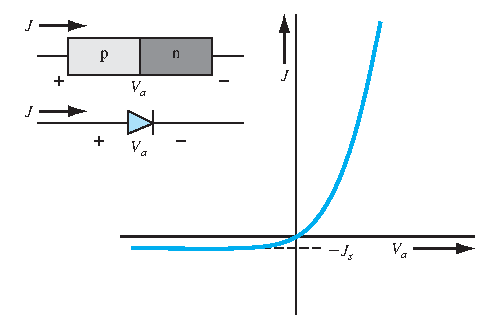
\includegraphics[width=0.5\linewidth]{./results/iv-curve_cropped.pdf}
    \caption{Ideal I-V characteristic of a p-n junction diode.}
    \label{textbook-iv-curve}
\end{figure}

\subsubsection{Shockley ideal diode equation}

The behavior of the current in both forward and reverse bias can be mathematically modeled by the Shockley Diode Equation (\ref{shockley}):

\begin{equation} \label{shockley}
I = I_0 (e^{\frac{qV}{nkT}}-1)
\end{equation}

Which, under normal forward bias operation, can be approximated to:

\begin{equation} \label{shockley-approx}
    I = I_0 (e^{frac{qV}nkT})
\end{equation}

Where $I_0$ is the reverse saturation current, $q$ is the charge of an electron, k is the Boltzmann constant, T is the absolute temperature in Kelvin, and n is the ideality factor (typically 1 for Germanium and 2 for Silicon).

The I-V curve can be generally divided into three regions: forward bias ($V$ \textgreater $\,\,0$), reverse bias ($V$ \textless $\,\,0$), and breakdown. This experiment will only focus on the forward bias region, where the applied potential reduces the width of the depletion region, allowing majority carriers to diffuse across the junction. In this region, the exponential term in Equation \ref{shockley} dominates, and the "-1" can be neglected for voltages V>3kT/q.


\subsubsection{Temperature dependency}

The performance of semiconductor devices is highly sensitive to thermal variations. In a p-n junction, temperature affects the I-V characteristic primarily through the intrinsic carrier concentration ($n_i$), which in turn dictates the reverse saturation current ($I_0$).

To understand how the forward voltage V changes with temperature T at a constant current I, we begin by rearranging the simplified Shockley equation (ignoring the '-1'):

\begin{equation}
V = \frac{nkT}{q} \ln\left(\frac{I}{I_0}\right)
\end{equation}

The reverse saturation current $I_0$ is strongly dependent on temperature because it is proportional to $n_i$. The relationship is given by:

\begin{equation}
I_0 \propto T^3 \exp\left(-\frac{E_g}{kT}\right)
\end{equation}

Where $E_g$ is the bandgap energy (approx. 1.12 eV for Silicon). Taking the derivative of the voltage expression with respect to temperature ($\frac{\delta V}{\delta T}$) while holding I constant involves accounting for both the linear T in the thermal voltage and the exponential T dependency within $I_0$. The resulting expression for the temperature coefficient is:

\begin{equation}
\label{eqn:temprelation}
\frac{dV}{dT} = \frac{V - (E_g/q)}{T} - \frac{3nk}{q}
\end{equation}

For a standard Silicon diode operating at room temperature with $E_g / q \approx 1.12 V$, the term ($V - E_g / q$) is negative. This yields the well-known approximation:

\begin{equation} 
\label{eqn:tempconst}
\frac{\delta V}{\delta T}|_{I = constant} \approx -2.4 \text{ mV/}^\circ\text{C}
\end{equation}

This negative temperature coefficient indicates that as the diode heats up, the potential barrier decreases, requiring less applied voltage to maintain the same level of current.

The temperature sensitivity of a p-n junction is fundamentally rooted in the thermal generation of charge carriers. While thermal voltage increases linearly with temperature, its effect is overshadowed by the exponential growth of the reverse saturation current $I_0$.

\subsubsection{Thermal Generation}

The reverse saturation current is defined by the minority carrier concentrations and their respective diffusion constants. Mathematically, $I_0$ is proportional to the square of the intrinsic carrier concentration ($n_i^2$):

\begin{equation}
I_0 \propto n_i^2 = B T^3 \exp\left(-\frac{E_g}{kT}\right)
\end{equation}

where B is a material-specific constant and $E_g$ is the energy bandgap. As temperature increases, more electrons gain sufficient thermal energy to overcome the bandgap, leading to an exponential increase in $n_i$. Because $I_0$ represents the "leakage" of minority carriers, an increase in T effectively lowers the barrier for carrier injection under forward bias.

For a constant forward current I, an increase in temperature allows that current to be achieved at a lower applied voltage V. This phenomenon results in a negative temperature coefficient for the forward voltage. By differentiating the diode equation, we find that for Silicon, the voltage required to maintain a specific current decreases by approximately 2.4 mV for every 1$^{\circ}$C increase in temperature.


\subsubsection{Built-in Potential}

Additionally, the built-in potential $V_{bi}$ of the junction also decreases with temperature:

\begin{equation}
V_{bi} = \frac{kT}{q} \ln\left(\frac{N_A N_D}{n_i^2}\right)
\end{equation}

As $n_i$ rises with temperature, the ratio inside the logarithm decreases faster than the linear T term increases. This reduction in the built-in barrier is the primary reason the I-V curve shifts toward the origin (left) as the device heats up.



\subsection{Light emitting diodes (LEDs)}

A Light Emitting Diode (LED) is a semiconductor p-n junction that converts electrical energy directly into light through a process known as electroluminescence. Unlike traditional light sources that rely on heat, LEDs are "cold" light sources, making them significantly more efficient.

\subsubsection{Mechanism of light emission}

When a forward-bias voltage is applied to the LED, electrons from the n-side and holes from the p-side are pushed toward the active region of the junction \cite{emission}.

\begin{enumerate}
\item Recombination: Electrons and holes meet and recombine.
    \vspace{-0.3\baselineskip}
\item Spontaneous Emission: As an electron moves from the higher-energy conduction band into a lower-energy hole in the valence band, it must release its excess energy.
    \vspace{-0.3\baselineskip}
\item Photon Release: In direct bandgap semiconductors, this energy is released as a photon. This process is called spontaneous emission because it occurs naturally without an external light trigger.
\end{enumerate}

\begin{figure}[!htbp]
    \centering
    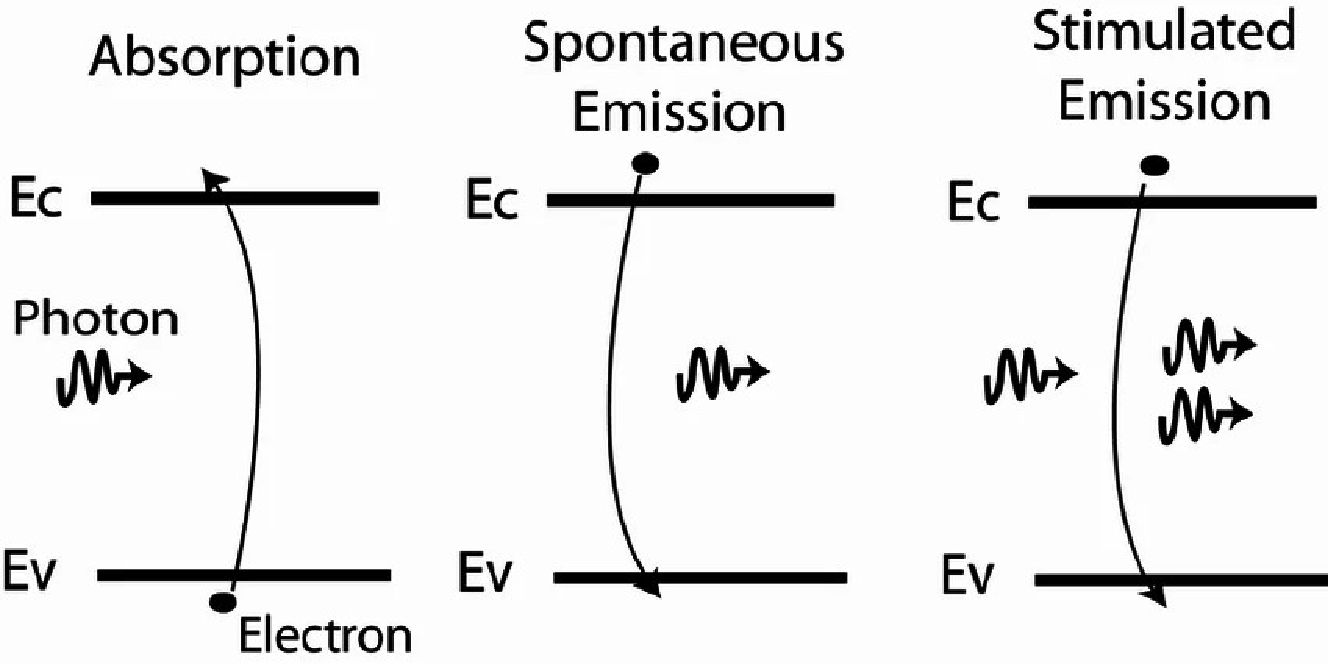
\includegraphics[width=0.65\linewidth]{./results/spontaneousemission.pdf}
    \caption{Illustration of absorption, spontaneous emission, and simulated emission}
\end{figure}


\subsubsection{The bandgap and light emission characteristics}

The energy of the emitted photon ($E$) is approximately equal to the bandgap energy ($E_g$) of the semiconductor material. This relationship is defined by the equation:

\begin{equation}
    \label{photon-energy}
    E = E_g = \frac{hc}{\lambda}
\end{equation}

Where $h$ is Planck's constant, $c$ is the speed of light, and $\lambda$ is the peak wavelength.

Because $E_g$ is an intrinsic property of the material, the peak wavelength, and thus the specific colour of the LED, is detemined by the choice of semiconductor material.

Additionally, while all semiconductors have a bandgap, not all are suitable for efficient light emission. This is determined by the alignment of the conduction band minimum and the valence band maximum in k-space (momentum space).

\begin{enumerate}
\item \textbf{Direct Bandgap:} The conduction band minimum and valence band maximum align at the same momentum ($k=0$). This allows electrons to recombine with holes and release energy directly as a \textbf{photon} without a change in momentum.
    \vspace{-0.3\baselineskip}
\item \textbf{Indirect Bandgap:} The band extrema are offset in momentum space. Recombination requires a third party—a phonon (lattice vibration)—to conserve momentum. This three-body interaction is inefficient, typically dissipating energy as \textbf{heat} rather than light.
\end{enumerate}

\subsubsection{Spectral characteristics}

LEDs are often described as monochromatic, but they differ significantly from other sources:

\begin{enumerate}
\item LED vs. Incandescent bulbs: Incandescent bulbs use blackbody radiation, emitting a broad "white" spectrum that includes infrared (heat). LEDs use a narrow band spectrum, concentrating their energy into a specific colour, which prevents energy waste.
    \vspace{-0.3\baselineskip}
\item Spectral Bandwidth: While narrow, LEDs are not perfectly monochromatic like lasers. They have a finite spectral linewidth (typically 20nm-50nm) due to the thermal distribution of carriers within the energy bands. 
\end{enumerate}

Table \ref{spectral-table} shows some examples of semiconductor materials used for optics fabrication \cite{Klimm:ro5002}. 

\begin{table}[!htbp]
    \label{spectral-table}
\centering
\caption{Semiconductor Materials and their Optical Characteristics}
\label{tab:led_materials}
\small % Slightly smaller font to ensure it fits the page width
\begin{tabular}{lllll}
\toprule
\textbf{Semiconductor Name} & \textbf{Composition} & \textbf{Wavelength (nm)} & \textbf{colour} & \textbf{Bandgap (eV)} \\ \midrule
Gallium Nitride & \ce{AlGaInN} & \textless 400 & Ultraviolet & 3.1--4.4 \\
Indium Gallium Nitride & \ce{InGaN} & 400--450 & Violet & 2.8--4.0 \\
Silicon Carbide & \ce{SiC}/\ce{InGaN} & 450--500 & Blue & 2.5--3.7 \\
Gallium Phosphide & \ce{AlGaInP}/\ce{GaP} & 500--570 & Green & 1.9--4.0 \\
Gallium Arsenide Phosphide & \ce{GaAsP} & 570--590 & Yellow & 2.1--2.2 \\
Alum. Gal. Indium Phosphide & \ce{AlGaInP} & 590--610 & Orange & 2.0--2.1 \\
Alum. Gallium Arsenide & \ce{AlGaAs}/\ce{GaAsP} & 610--760 & Red & 1.6--2.0 \\
Gallium Arsenide & \ce{GaAs} & \textgreater 760 & Infrared & \textless 1.9 \\ \bottomrule
\end{tabular}
\end{table}


\subsubsection{Factors affecting the spectrum}

The output of an LED is not static; it can be shifted by environmental and operational factors:

\begin{enumerate}
\item Temperature Sensitivity: As the junction temperature increases, the semiconductor bandgap typically narrows. This causes a red-shift (longer wavelength) in the peak emission and a decrease in overall intensity.
    \vspace{-0.3\baselineskip}
\item Current Density: Increasing the drive current can cause a slight "blue-shift" in some materials due to band-filling effects, though this is often offset by the heat generated by the higher current.
\end{enumerate}


\section{Experimental Technique}

\subsection{I-V characteristics}

\begin{figure}[!htbp]
    \centering
    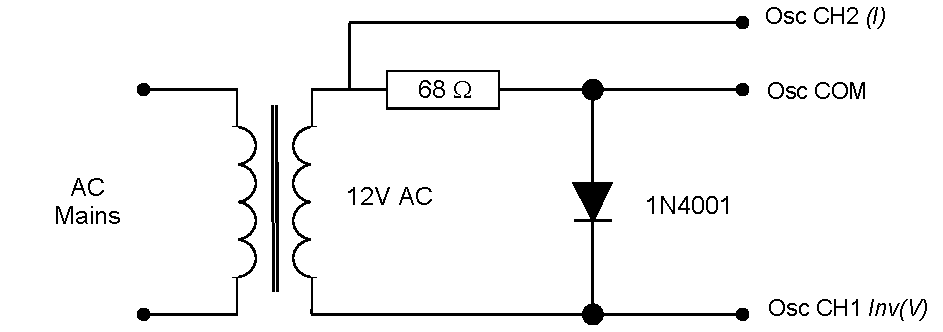
\includegraphics[width=0.7\linewidth]{./results/ivdisplay_cropped.pdf}
    \caption{Sweep circuit for I-V display}
    \label{iv-display}
\end{figure}

To observe the forward-bias I-V characteristic of a 1N4001 diode, a circuit \ref{iv-display} was constructed using a 12V AC source and a $68 \Omega$ resistor. The diode's response was monitored via an oscilloscope set to X-Y mode, with the origin properly calibrated. The current range was adjusted to ensure visibility of measurements exceeding 150 mA. From the resulting curve, the turn-on voltage and differential resistance (dV/dI) post-turn-on were determined \cite{labmanual}.


\subsection{Temperature Dependence}

The thermal sensitivity of the p-n junction was tested by applying localized heat to the diode using a soldering iron for approximately 15 seconds. Precautionary measures were taken to ensure the $68 \Omega$ resistor remained unheated. The shifted I-V characteristic was recorded, and the voltage shift at a constant current of 150 mA was measured in millivolts. This data was then used to calculate the actual temperature change ($\Delta T$) of the diode in Kelvin \cite{labmanual}.


\subsection{Ideality factor and reverse saturation current}

\begin{figure}[!htbp]
    \centering
    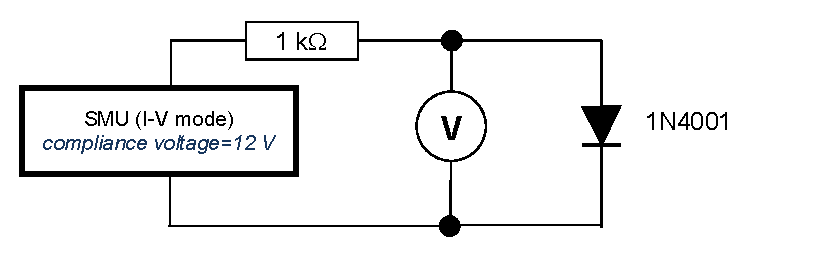
\includegraphics[width=0.7\linewidth]{./results/diodeparameter_cropped.pdf}
    \caption{Circuit for diode parameter extraction}
    \label{parameter-extraction}
\end{figure}

For a more precise extraction of the ideality factor ($n$) and reverse saturation current ($I_0$), a separate circuit was utilized to measure the characteristic over three decades of current (0.01 mA to 10 mA). A Source Measure Unit (SMU) was used to record current values while a Digital Multimeter (DMM) measured the corresponding voltage. The resulting data were plotted on a semi-logarithmic scale ($\ln{I}$ vs. V) to determine n and  $I_0$ from the slope and intercept of the linear region. \cite{labmanual}


\subsection{Light current characteristic of an LED}

\begin{figure}[!htbp]
    \centering
    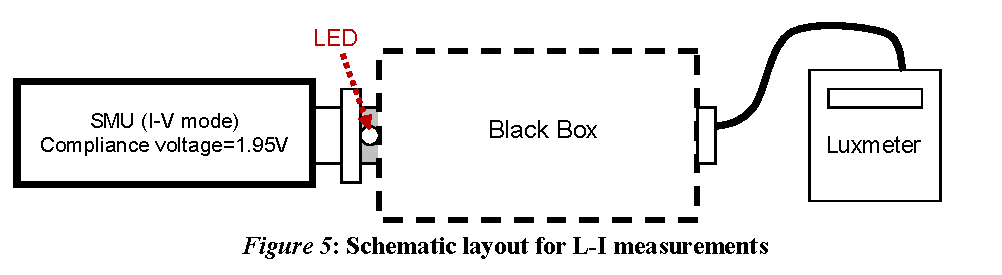
\includegraphics[width=0.7\linewidth]{./results/schematic-layout_cropped.pdf}
    \caption{Schematic layout for L-I measurements}
    \label{l-i-measurements}
\end{figure}

The L-I characteristics of an ultra-bright red LED were measured using a setup consisting of an SMU and a luxmeter placed within a black box, as shown in \ref{l-i-measurements} \cite{labmanual}. The SMU provided a constant DC current, which was increased from 0 to 35 mA in 5 mA increments. The corresponding optical power, proportional to the luxmeter readings, was recorded for each step to characterize the linearity of the light emission.

The experiment must be carried out inside the black box so as to block out ambient light, such that the luxmeter strictly measures optical power resulting from the light emitted by the LEDd. This maximises the signal-to-noise ratio (SNR).

\subsection{Emission spectrum of an LED}

\begin{figure}[!htbp]
    \centering
    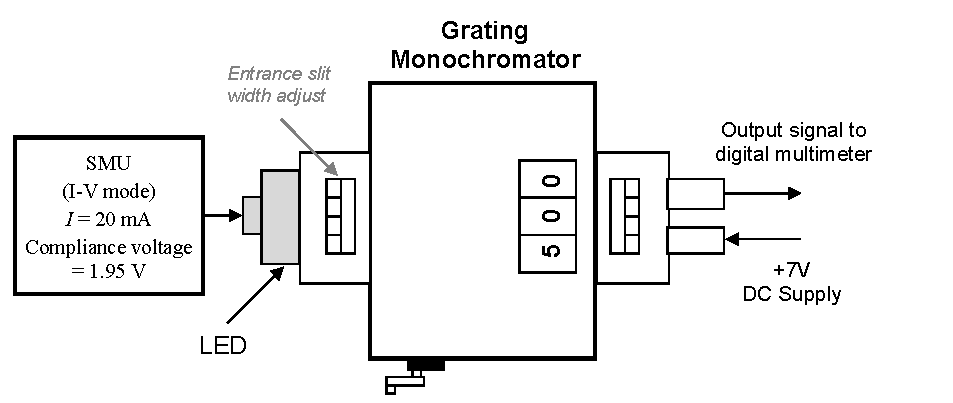
\includegraphics[width=0.7\linewidth]{./results/gratingmonochromator_cropped.pdf}
    \caption{Measurement of emission spectrum using a grating spectrometer}
    \label{monochromator}
\end{figure}

The spectral properties of the LED were analyzed using a grating spectrometer, as illustrated in figure.\ref{monochromator} \cite{labmanual}. With the LED biased at a constant 20 mA, the reflective grating was rotated to disperse the emitted light into its constituent wavelengths. A photodetector, powered by a 7V DC supply and connected to a voltmeter, measured the light intensity at specific wavelength intervals between 600 nm and 700 nm. This data allowed for the determination of the peak emission wavelength, the semiconductor energy bandgap ($E_g$), and the full width at half maximum (FWHM) linewidth. 


\section{Results and Discussions}

\subsection{Finding ideality factor and reverse saturation current of diode}

\begin{figure}[!htbp]
    \centering
    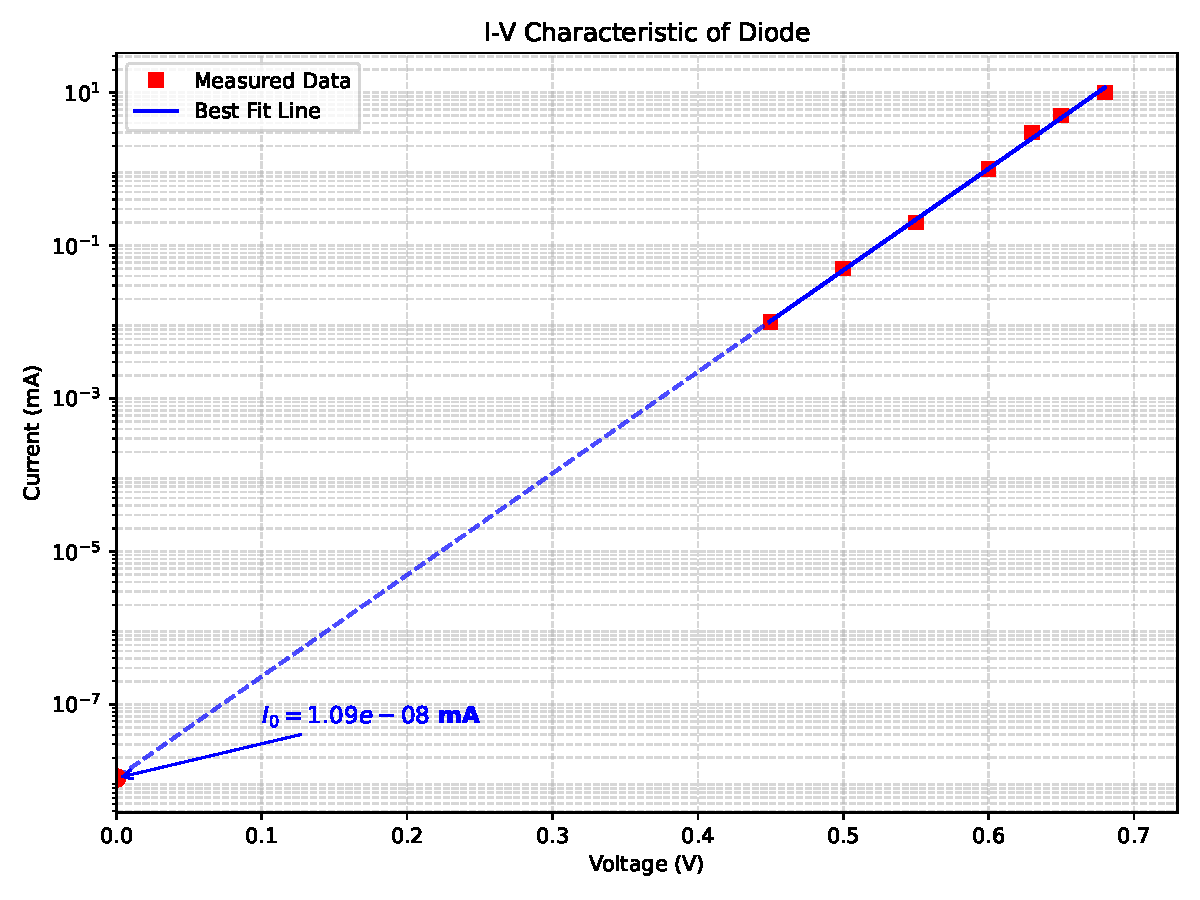
\includegraphics[width=0.8\linewidth]{./results/iv-curve-semilog.pdf}
    \caption{$\ln{I}$ (A) plotted against voltage (V)}
    \label{iv-semilog}
\end{figure}

By taking the natural logarithm of both sides of the equation ( ref{shockley-approx} ), a linear expression (visualised in figure.\ref{iv-semilog}) can be derived:

\begin{equation} 
\ln{I} = \ln{I_0} + \frac{q}{nkT}V
\end{equation}

where the gradient can be expressed as:

\begin{equation}
m = \frac{\ln{I_2} - \ln{I_1}}{V_2 - V-1}
\end{equation}

which can then be used to find the ideality factor $n$ through:

\begin{equation}
n = \frac{q}{mkT}
\end{equation}

From the extrapolated linear best-fit line, $m$ is determined to be $30.6$ (3 s.f.). Taking room temperature to be $25^\circ C$, or $298 K$, the following result can be obtained:

\begin{equation} \label{ideality}
n = 1.27
\end{equation}


\subsection{I-V characteristics of diode under temperature variation}

\begin{figure}[!htbp]
    \centering
    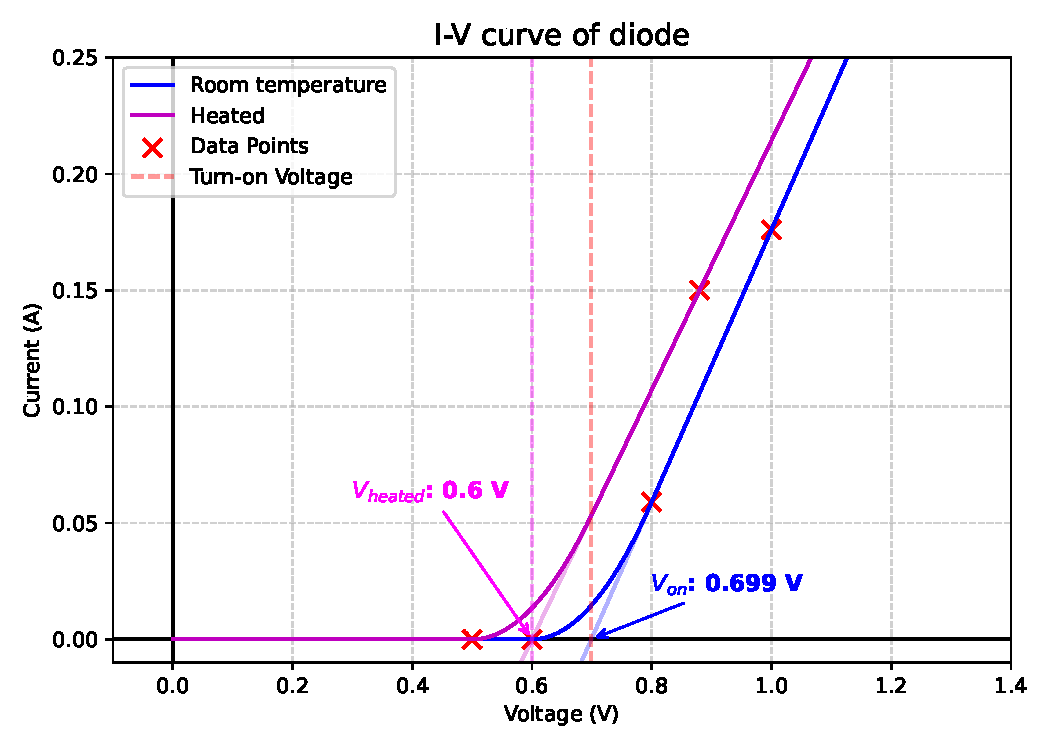
\includegraphics[width=0.8\linewidth]{./results/iv-sketch.pdf}
    \caption{Sketch of IV curve of diode, at room temperature and with heating}
    \label{iv-sketch}
\end{figure}    

\begin{figure}[!htbp]
    \centering
    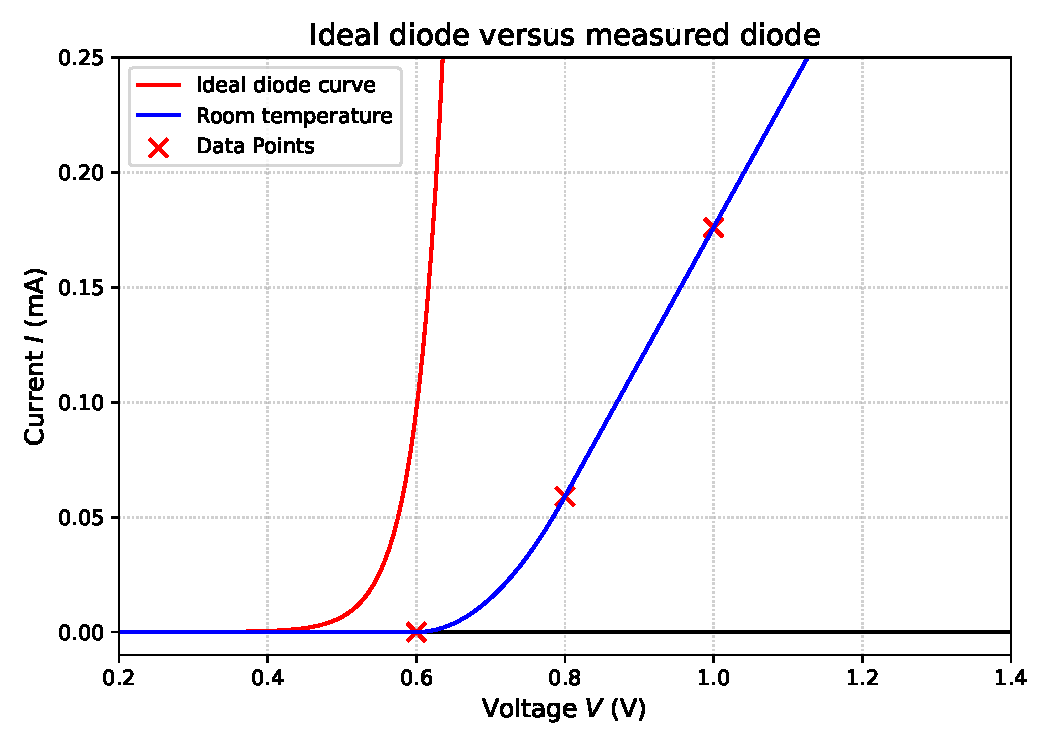
\includegraphics[width=0.8\linewidth]{./results/ideal-iv.pdf}
    \caption{Ideal shockley diode I-V characteristics plotted with measured diode I-V characteristics at room temperature}
    \label{iv-ideal}
\end{figure}    

The experimental values for the I-V characteristics of the diode at both room temperature and when heated are visualised on figure.\ref{iv-sketch}. The ideal diode modelled with \ref{shockley} is visualised on figure. \ref{iv-ideal}.

From figure.\ref{iv-sketch}, it can be seen that the turn-on voltages of the diode at room temperature and after heating are approximately 0.7 V and 0.6 V. The voltage shift at constant 150 mA current is about -90 mV. 

By using equations ( \ref{eqn:tempconst} ) and ( \ref{eqn:temprelation} ), an expression for $\Delta T$ can be formed:

\begin{equation}
\Delta T = \frac{\Delta V (mV)}{-2.4 (mV/K)}
\end{equation}

Subsituting the values from the sketch into the expression above, $\Delta T$ is found to be $\approx$ 37.5 K. 


\subsubsection{Shockley ideal diode and observed diode characteristics}

The observed disparity between the measured I-V characteristics and the Shockley model, even after using the extracted parameters $n$ and $I_0$ in the Shockley ideal diode equation, can be attributed to several non-ideal noise factors. At higher current levels, the curve begins to deviate from the exponential model and appears to becomes more linear; this is primarily due to the internal series resistance ($R_s$) of the diode's intrinsic material and ohmic contacts, which creates an additional voltage drop not accounted for in Equation \ref{shockley}. Additionally, high-injection effects and localized self-heating during measurement likely caused the actual junction temperature to rise slightly above the ambient room temperature, leading to an increase in the reverse saturation current $I_0$ beyond the initial measured value.


\subsubsection{Factors determining the turn-on voltage of a p-n junction diode}

The turn-on voltage ($V_{on}$) of a p-n junction is not a fixed physical constant but is defined by the point at which the forward bias sufficiently reduces the potential barrier to allow significant carrier injection. It is primarily determined by the following factors:

\begin{enumerate}
    \item \textbf{Semiconductor Material and Bandgap ($E_g$):} 
    The most fundamental factor is the energy bandgap of the semiconductor. The built-in potential ($V_{bi}$), which $V_{on}$ must overcome, is directly related to the energy required to move carriers across the junction. For instance, silicon diodes typically have a $V_{on}$ of approximately 0.6-0.7 V, whereas wide-bandgap materials like those used in LEDs require significantly higher voltages (e.g., ~1.8-2.0 V for red LEDs) to initiate conduction \cite{Yoshikawa2007}.
    
    \item \textbf{Doping Concentrations ($N_A$ and $N_D$):} 
    The magnitude of the built-in potential is mathematically defined by the doping levels on the p-side ($N_A$) and n-side ($N_D$):
    \begin{equation}
        V_{bi} = \frac{kT}{q} \ln \left( \frac{N_A N_D}{n_i^2} \right)
    \end{equation}
    Higher doping concentrations increase the density of majority carriers, which widens the separation between Fermi levels in the neutral regions. This results in a larger $V_{bi}$ and a corresponding increase in the voltage required to drive a significant current through.

    \item \textbf{Temperature dependence:} 
    The turn-on voltage is highly sensitive to temperature ($T$). As temperature increases, the intrinsic carrier concentration ($n_i$) increases exponentially. This causes a significant increase in the reverse saturation current ($I_0$), which effectively lowers the potential barrier[cite: 1]. Experimentally, this is observed as a leftward shift in the I-V characteristic, with $V_{on}$ typically decreasing at a rate of approximately $-2.4$ mV/K for silicon devices \cite{silicon-temp}.
\end{enumerate}


\subsection{Light-current curve}

\begin{figure}[!htbp]
    \centering
    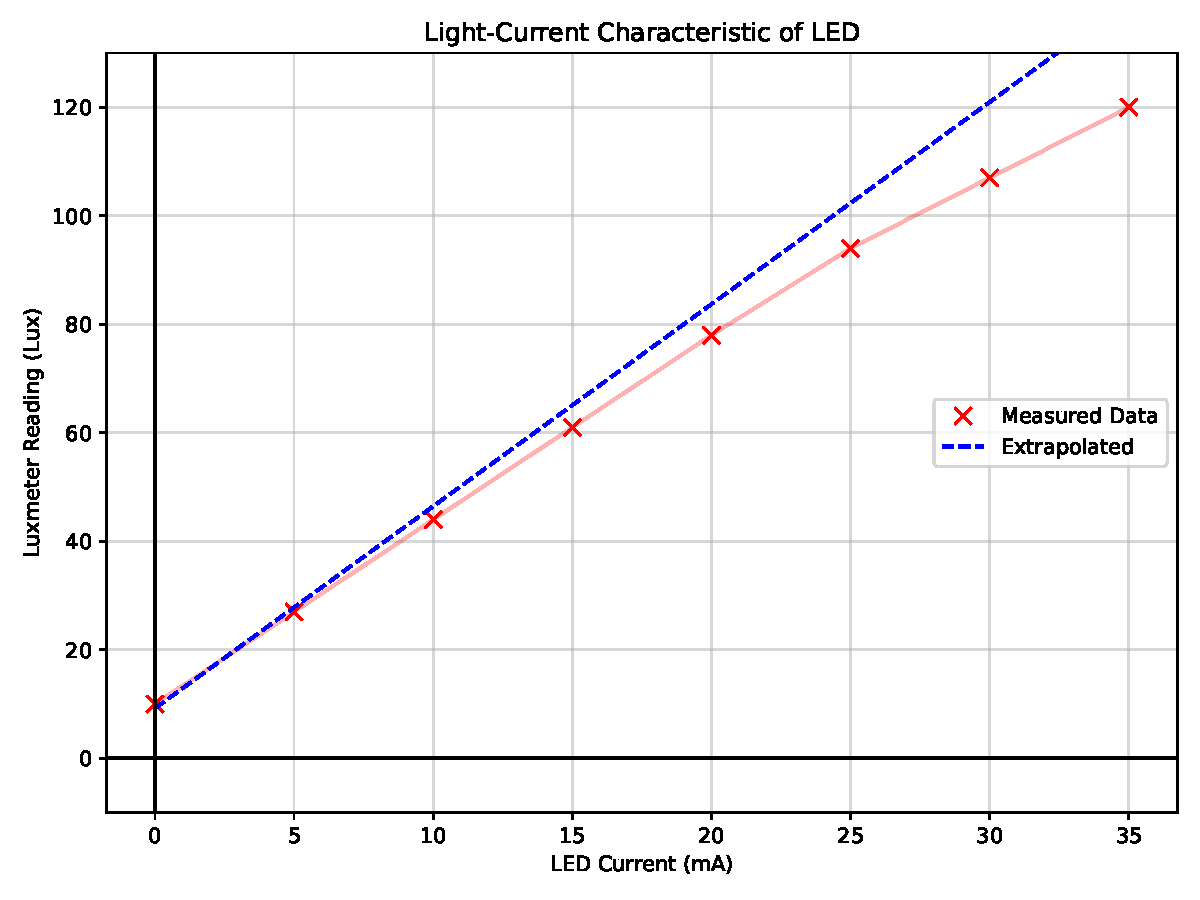
\includegraphics[width=0.8\linewidth]{./results/light_current_curve.pdf}
    \caption{Light intensity plotted against current through the LED.}
    \label{light-current}
\end{figure}

When the LED current was 0 mA, a luxmeter reading of 10 Lux was observed. Theoretically, at zero bias, there is no carrier injection and thus zero spontaneous emission. However, this was not the case in the experiment. The non-zero reading can be attributed to several factors: and there are a few possible reasons for the nonzero reading: it could be due to ambient light leaked into the black box, dark current due to sensor thermal noise, or residual phosophorescence from the phosphor coating on the LED bulb surface.

\subsubsection{Observed change in the gradient of the measured L-I curve at large currents}

The experimental L-I curve (Figure \ref{light-current}) ideally follows a linear relationship, $L \propto I_F$. However, at higher injection currents ($>25$ mA), a sub-linear trend or "droop" in the gradient is observed. This decrease in external quantum efficiency is attributed to several competing non-radiative processes:

\begin{enumerate}
    \item \textbf{Joule Heating and Thermal Quenching:} 
    As forward current increases, power dissipation within the series resistance ($R_s$) and the junction itself leads to significant localized heating ($P = I^2 R_s + IV_{j}$). This rise in junction temperature reduces the internal quantum efficiency in two ways:
    \begin{itemize}
        \item It increases the probability of \textbf{phononic vibrations}, which assist non-radiative transitions where carrier energy is dissipated as heat rather than light.
        \item It facilitates \textbf{carrier overflow}, where high-energy electrons escape the active region before they can recombine radiatively.
    \end{itemize}

    \item \textbf{Auger Recombination:} 
    Unlike radiative recombination, which involves an electron and a hole, Auger recombination is a three-particle process. In this mechanism, the energy released by the recombination of an electron-hole pair is transferred to a third carrier (either an electron in the conduction band or a hole in the valence band), which is excited to a higher energy state. Because the probability of this event scales with the \textbf{cube of the carrier density} ($C \cdot n^3$), it becomes a dominant loss mechanism only at high injection levels, causing the light output to lag behind the increase in current.

    \item \textbf{Shockley-Read-Hall (SRH) Recombination:} 
    SRH recombination occurs when carriers are captured by deep-level defects or impurities within the forbidden bandgap. While typically dominant at \textit{low} currents, the overall increase in total recombination rate at high currents includes a non-radiative SRH component. As the injection level increases, the saturation of radiative states can cause a higher proportion of carriers to be lost to these trap-assisted non-radiative centers, further contributing to the degradation of the L-I slope \cite{shockley-read-hall}.
\end{enumerate}

\subsection{Emission spectrum of LED}

\begin{figure}[!htbp]
    \centering
    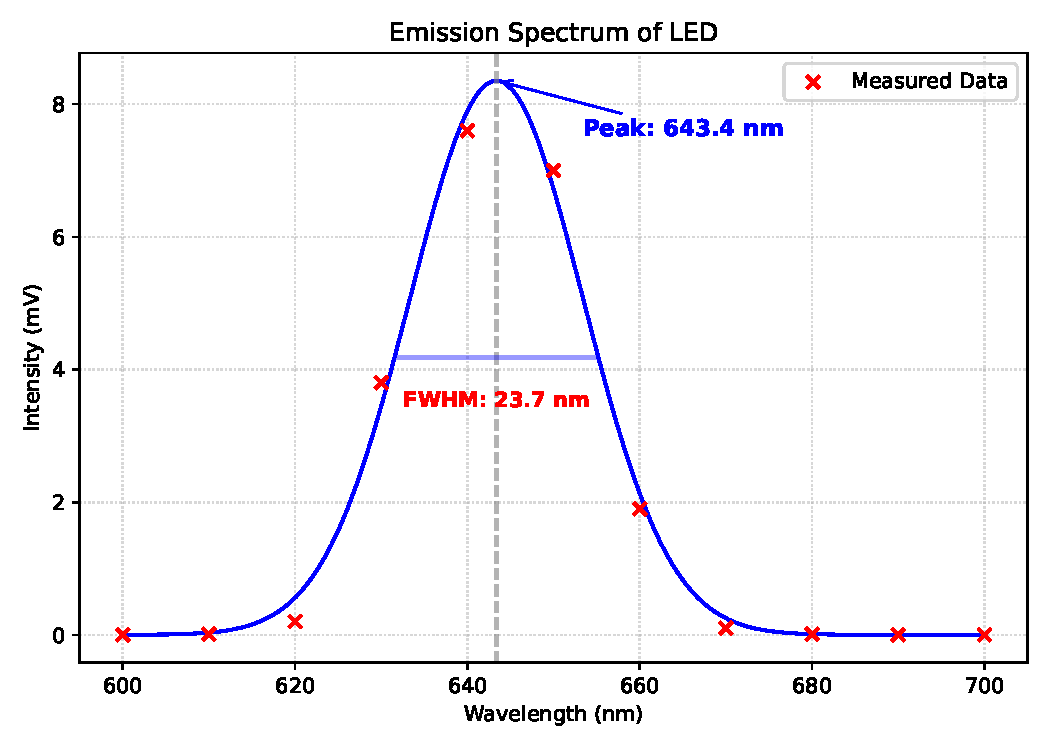
\includegraphics[width=0.8\linewidth]{./results/emission_spectrum.pdf}
    \caption{Light intensity plotted against emission wavelength of LED.}
    \label{emission-spectrum}
\end{figure}

Unlike incandescent light devices, which emit light through blackbody radiation and thus emits light of all wavelengths (white light), LEDs emit light through spontaneous emission, as previously discussedm and thus has a narrow-band spectrum (single colour light).

The peak wavelength of light emitted by the LED Is determined by the bandgap energy $E_g$. Additionally, LEDs have a spectral bandwidth, as they are not perfectly monochromatic like lasers.

The peak wavelength of the LED used in this experiment is 643.4 nm, as seen from figure.\ref{emission-spectrum}.

\vspace{0.6\baselineskip}

Two factors affecting the emission spectrum could be:

\begin{enumerate}
    \item Temperature sensitivity: the greater the temperature, the smaller the bandgap energy $E_g$, and hence the greater the peak wavelength. This phenemonon is also called \textbf{redshift}.
    \vspace{-0.3\baselineskip}
    \item Current density: the greater the current, the greater the band-filling effect, and the shorter the peak wavelength. This phenomenon is called \textbf{blueshift}. However, it should be noted that blueshift has a negligible effect on the emission spectrum of the LED, and thus is often masked by the redshift effect.
\end{enumerate}

\subsubsection{Factors influencing the spectral line width of the measured LED emission spectrum}

The measured emission spectrum (Figure \ref{emission-spectrum}) exhibited a Full Width at Half Maximum (FWHM) of 23.7 nm. Unlike the near-monochromatic emission of a laser, LED emission is characterized by a broader spectral width, which is primarily influenced by the following physical factors:

\begin{enumerate}
    \item \textbf{Thermal Distribution of Carriers (Thermal Broadening):} 
    The most significant factor determining the linewidth is the energy distribution of electrons and holes within their respective bands. According to Fermi-Dirac statistics, carriers do not all occupy the very bottom of the conduction band or the very top of the valence band; instead, they are distributed over an energy range of approximately $3kT$. Because recombination can occur between carriers at various energy levels within this thermal distribution, the resulting photons possess a spread of energies ($\Delta E \approx 3kT$), leading to a broader spectral peak.

    \item \textbf{Alloy Fluctuations and Material Inhomogeneity:} 
    Red LEDs are typically fabricated from ternary or quaternary alloys such as AlGaInP[cite: 11]. On a microscopic scale, the distribution of these elements may not be perfectly uniform. Small local fluctuations in the material composition lead to slight variations in the local bandgap energy ($E_g$) across the active region. These varying local bandgaps result in a range of emission wavelengths that combine to broaden the overall measured spectrum.

    \item \textbf{Heavy Doping and Band Tailing:} 
    High doping concentrations used to improve device conductivity can cause "band tailing," where the high density of impurities creates a continuum of states that extend into the forbidden bandgap. Radiative transitions involving these tail states occur at energies slightly lower than the nominal $E_g$, adding a "red-shifted" shoulder to the spectrum and increasing the FWHM.

    \item \textbf{Self-Heating Effects:} 
    During operation, non-radiative recombination and series resistance generate heat within the junction. As the junction temperature rises, the carrier thermal distribution ($3kT$) widens, and the bandgap typically narrows. Both effects contribute to a wider and slightly shifted emission spectrum compared to low-power or pulsed operation.
\end{enumerate}


\section{Conclusion}

In this experiment, the electrical and optical properties of p-n junction devices were investigated, showing satisfiable agreement with established semiconductor theory. The diode displayed the expected exponential I-V behaviour under forward bias, with deviations attributed to non-ideal effects such as series resistance and self-heating. Temperature variation further highlighted the strong influence of thermal effects, reducing the effective potential barrier and shifting the I-V characteristics. For the LED, the light-current relationship was linear at low currents but deviated at higher currents due to non-radiative recombination, reducing efficiency. The emission spectrum also confirmed that LED light is not perfectly monochromatic, with its finite width arising from intrinsic material and thermal effects. 

Overall, the results demonstrate how fundamental semiconductor principles govern device behaviour while emphasising the impact of real-world non-idealities.

\section{References}

\printbibliography

\end{document}